\documentclass[aspectratio=169]{beamer}

\usepackage{amsmath,amssymb,amsfonts,amsthm}
\usepackage[T1]{fontenc}
\usepackage[utf8]{inputenc}
\usepackage[english]{babel}
\usepackage{hyperref}
\usepackage{lmodern}
\usepackage{comment}
\usepackage{xcolor}
\usepackage{graphicx,subcaption}
\usepackage{tikz,float}
\usepackage{pgfplots}
\usepackage{expl3}

\usetikzlibrary{positioning, fit}
\usepackage{tcolorbox}

\renewcommand{\epsilon}{\varepsilon}
\newcommand{\R}{\mathbb{R}}
\newcommand{\N}{\mathbb{N}}
\newcommand{\B}[2]{\mathcal{B}_{#1}\left(#2\right)}
\newcommand{\todo}[1]{{\color{red}#1}}

% Use Unipd as theme, with options:
% - pageofpages: define the separation symbol of the footer page of pages (e.g.: of, di, /, default: of)
% - logo: position another logo near the Unipd logo in the title page (e.g. department logo), passing the second logo path as option 
% Use the environment lastframe to add the endframe text
\usetheme[pageofpages=of]{Unipd}
\usefonttheme[onlymath]{serif}

\title{Random subsampling techniques for sea bass mortality prediction}
\author{Giovanni Gaio, Simone Moretti}
\date{\today}
\subtitle{}

\date{\today}

\begin{document}

\frame{\titlepage}

\begin{frame}
\frametitle{Overview}
%TODO change all

\begin{itemize}
  \item Motivation: Identifying impactful SNPs in sea bass mortality
  \item Dataset: Genomic SNP data, mortality outcomes, and annotations
  \item Method: Subsampling techniques with XGBoost
  \item Results: Accuracy/F1 vs. subsampling rate
  \item Conclusion: Subsampling preserves predictive power
\end{itemize}
\end{frame}

\begin{frame}
\frametitle{VNN and Sea Basses}

\begin{minipage}{0.49\textwidth}
  \textbf{Viral nervous necrosis} (\textbf{VNN}) is a highly spread disease among sealife.

\end{minipage}
\begin{minipage}{0.49\textwidth}
    \centering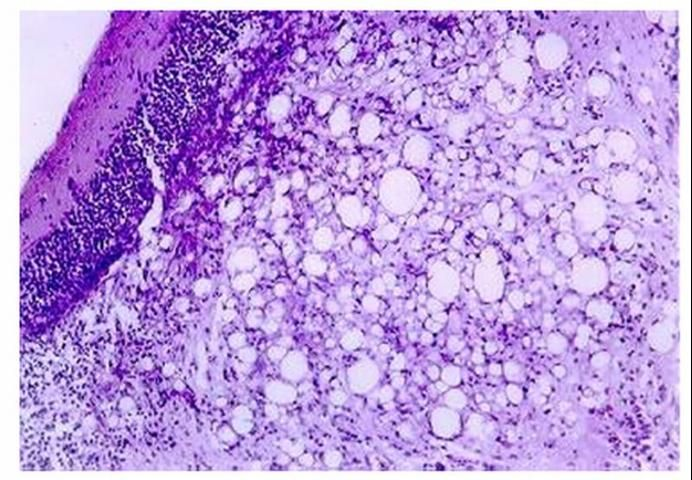
\includegraphics[width=0.7\linewidth]{figures/VNN.jpg}
\end{minipage}

\begin{minipage}{0.49\textwidth}
    \centering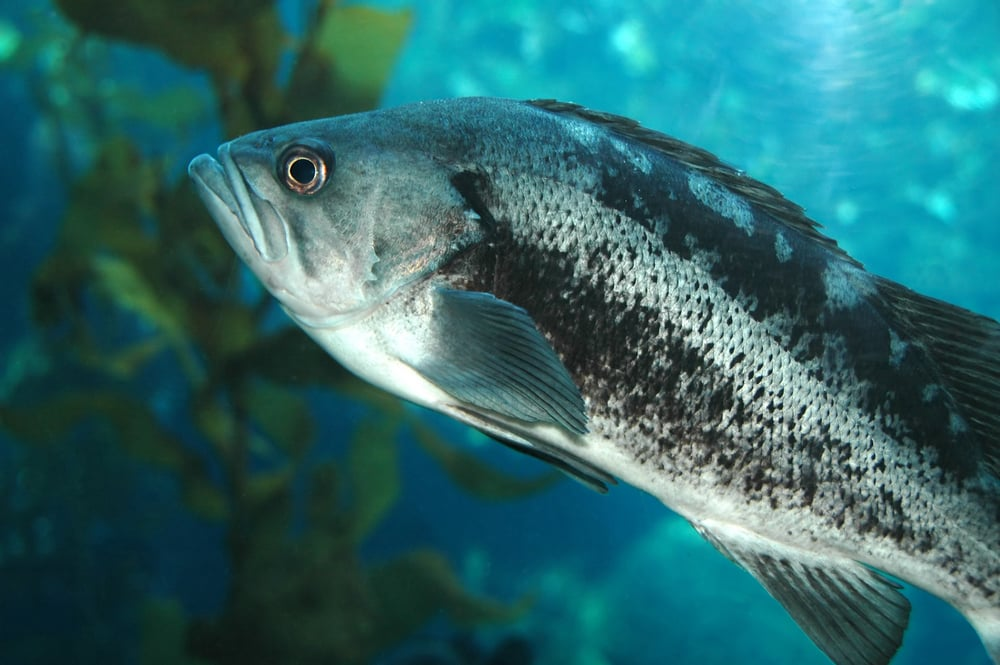
\includegraphics[width=0.7\linewidth]{figures/Black-Sea-Bass-303435837.jpg}
\end{minipage}
\begin{minipage}{0.49\textwidth}
  We concentrate our efforts on predicting the mortality of a population of \textbf{sea basses} affected by VNN.
\end{minipage}

\end{frame}

\begin{frame}
\frametitle{SNPs for predicting mortality}  

\begin{minipage}[c]{0.45\textwidth}
  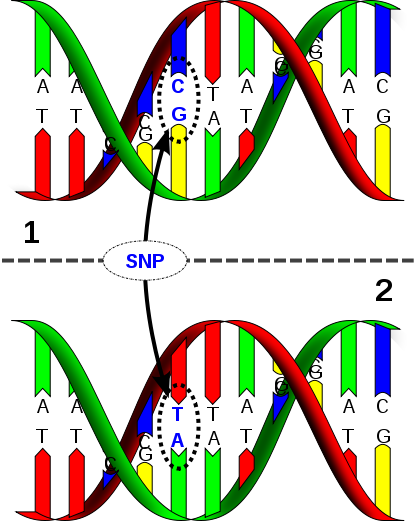
\includegraphics[width=0.8\linewidth]{figures/SNP.png}
\end{minipage}
\begin{minipage}[c]{0.5\textwidth}

  The \textbf{genome} might be useful to predict mortality.

  \vspace{1cm}

  \textbf{SNPs}: Single nucleotide polymorphisms.

\end{minipage}
\end{frame}


\begin{frame}
\frametitle{Machine Learning Approach}
%TODO change layout
  Predict if a sea bass will die by watching its genome: \textbf{Machine Learning}.

\vspace{0.3cm}

\begin{minipage}[c]{0.5\textwidth}
  In particular, we use the \textbf{XGBoost} classifier.
\end{minipage}
\begin{minipage}[c]{0.45\textwidth}
  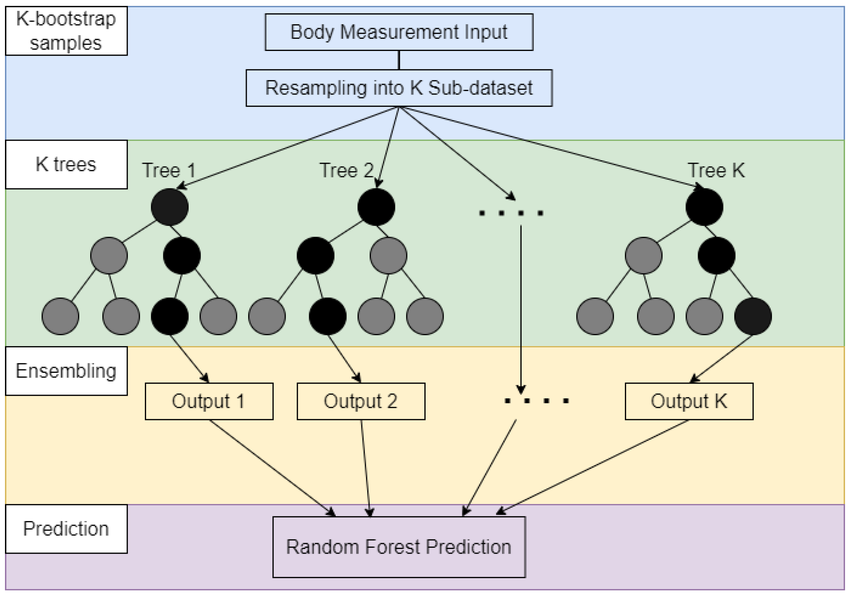
\includegraphics[width=0.9\linewidth]{figures/xggoost.png}
\end{minipage}
\end{frame}


\begin{frame}
\frametitle{Challenges with Genomic Data}
\begin{minipage}[c]{0.5\textwidth}
\begin{itemize}
  \item Each fish: over \textbf{6 million} SNP positions.
  \item Sample size: only \textbf{990} sea bass individuals.
  \item Traditional models may \textbf{overfit} due to high dimensionality.
  \item We mitigate through \textbf{subsampling}.
\end{itemize}
\end{minipage}
\begin{minipage}[c]{0.49\textwidth}
  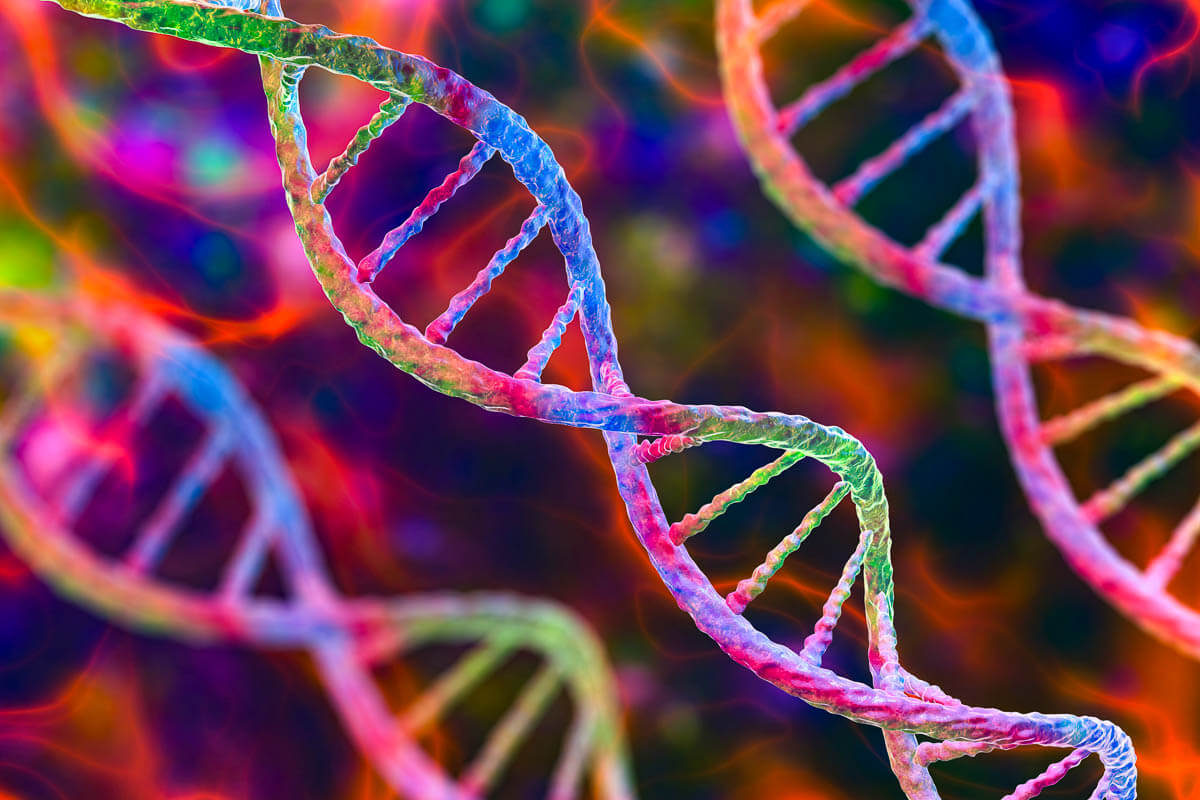
\includegraphics[width=\linewidth]{figures/dna.jpg}
\end{minipage}
\end{frame}

\begin{frame}{Pipeline Overview}
\begin{figure}[htb!]
    \centering
    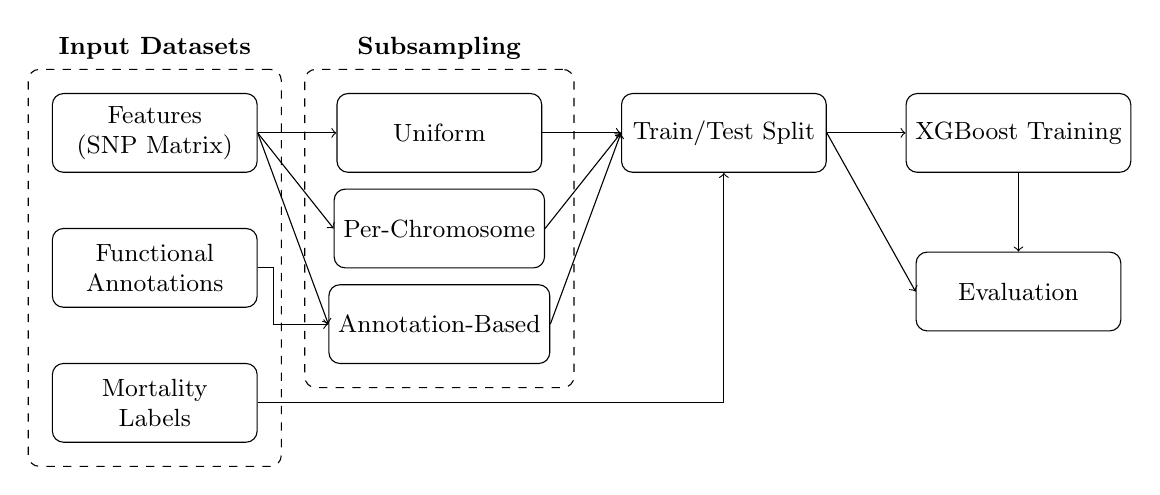
\begin{tikzpicture}[
        node distance=1cm and 0.1cm,
        every node/.style={font=\small},
        box/.style={draw, rectangle, rounded corners, minimum height=1cm, minimum width=2.6cm, align=center},
        group/.style={draw, rectangle, dashed, inner sep=0.3cm, rounded corners}
    ]

    \node[box] (features) {Features \\ (SNP Matrix)};
    \node[box, below=0.7cm of features] (annotation) {Functional \\ Annotations};
    \node[box, below=0.7cm of annotation] (mortality) {Mortality \\ Labels};

    \node[group, fit=(features)(mortality)(annotation), label=above:{\textbf{Input Datasets}}] (dataset_group) {};

    \node[box, right=1cm of features] (uniform) {Uniform};
    \node[box, below=0.2cm of uniform] (chr) {Per-Chromosome};
    \node[box, below=0.2cm of chr] (annot) {Annotation-Based};

    \node[group, fit=(uniform)(chr)(annot), label=above:{\textbf{Subsampling}}] (subsampling_group) {};

    \node[box, right=1cm of uniform] (split) {Train/Test Split};
    \node[box, right=1cm of split] (xgboost) {XGBoost Training};
    \node[box, below=of xgboost] (evaluate) {Evaluation};

    \draw[->] (features.east) -- ++(0.1,0) |- (uniform.west);
    \draw[->] (features.east) -- (chr.west);
    \draw[->] (features.east) -- (annot.west);

    \draw[->] (annotation.east) -- ++(0.2,0) |- (annot.west);

    \draw[->] (uniform.east) -- ++(0.1,0) |- (split.west);
    \draw[->] (chr.east) -- (split.west);
    \draw[->] (annot.east) -- (split.west);

    \draw[->] (mortality.east) -| (split.south);

    \draw[->] (split.east) -- (xgboost.west);
    \draw[->] (split.east) -- (evaluate.west);
    \draw[->] (xgboost.south) -- (evaluate.north);

    \end{tikzpicture} % \caption{Pipeline of the model training after subsampling of the data}
    \label{fig:pipeline}
\end{figure}
\end{frame}

\begin{frame}{Input Datasets}
\begin{figure}[htb!]
    \centering
    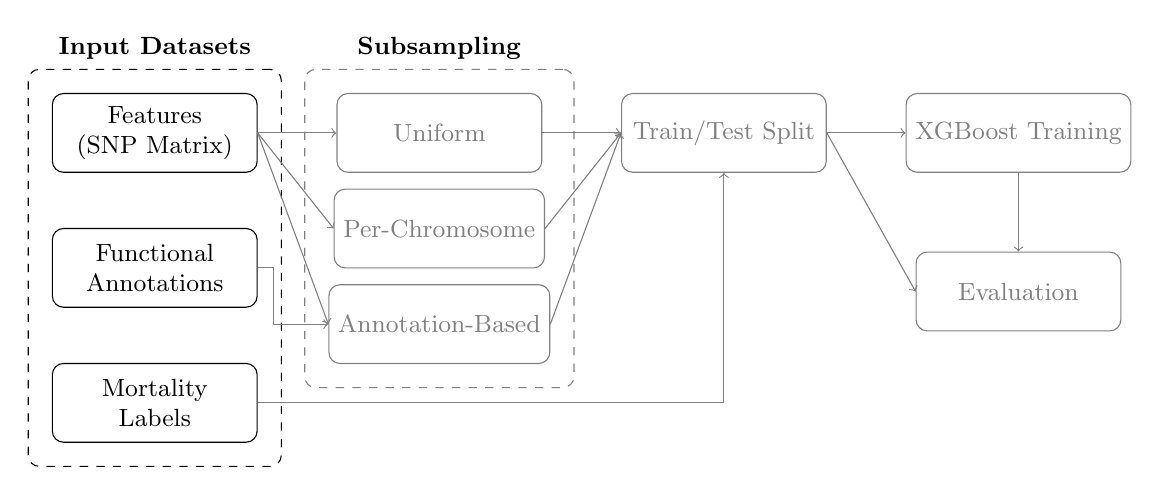
\begin{tikzpicture}[
        node distance=1cm and 0.1cm,
        every node/.style={font=\small},
        box/.style={draw, rectangle, rounded corners, minimum height=1cm, minimum width=2.6cm, align=center},
        group/.style={draw, rectangle, dashed, inner sep=0.3cm, rounded corners}
    ]

    \node[box] (features) {Features \\ (SNP Matrix)};
    \node[box, below=0.7cm of features] (annotation) {Functional \\ Annotations};
    \node[box, below=0.7cm of annotation] (mortality) {Mortality \\ Labels};

    \node[group, fit=(features)(mortality)(annotation), label=above:{\textbf{Input Datasets}}] (dataset_group) {};

    \node[box, color=gray, right=1cm of features] (uniform) {Uniform};
    \node[box, color=gray, below=0.2cm of uniform] (chr) {Per-Chromosome};
    \node[box, color=gray, below=0.2cm of chr] (annot) {Annotation-Based};

    \node[group, color=gray, fit=(uniform)(chr)(annot), label=above:{\textbf{Subsampling}}] (subsampling_group) {};

    \node[box, color=gray, right=1cm of uniform] (split) {Train/Test Split};
    \node[box, color=gray, right=1cm of split] (xgboost) {XGBoost Training};
    \node[box, color=gray, below=of xgboost] (evaluate) {Evaluation};

    \draw[->, color=gray] (features.east) -- ++(0.1,0) |- (uniform.west);
    \draw[->, color=gray] (features.east) -- (chr.west);
    \draw[->, color=gray] (features.east) -- (annot.west);

    \draw[->, color=gray] (annotation.east) -- ++(0.2,0) |- (annot.west);

    \draw[->, color=gray] (uniform.east) -- ++(0.1,0) |- (split.west);
    \draw[->, color=gray] (chr.east) -- (split.west);
    \draw[->, color=gray] (annot.east) -- (split.west);

    \draw[->, color=gray] (mortality.east) -| (split.south);

    \draw[->, color=gray] (split.east) -- (xgboost.west);
    \draw[->, color=gray] (split.east) -- (evaluate.west);
    \draw[->, color=gray] (xgboost.south) -- (evaluate.north);

    \end{tikzpicture}
\end{figure}
\end{frame}

\begin{frame}
\frametitle{SNP Dataset Structure}
\begin{minipage}{0.69\textwidth}
\begin{itemize}
  \item 990 rows (fish), each with 6,072,853 SNP features.
  \item SNP values: 0 (no mutation), 1 (heterozygous), 2 (homozygous alt).
  \item Each fish is paired with a mortality label.
\end{itemize}
\end{minipage}
\begin{minipage}{0.28\textwidth}
\resizebox{\textwidth}{!}{
\begin{tabular}{c|c}
\textbf{id} & \textbf{mortality} \\
\hline
PL06-B12 & 1 \\
PL06-B06 & 1 \\
PL06-E06 & 1 \\
PL08n-B05 & 0 \\
PL08n-G09 & 0 \\
$\vdots$ & $\vdots$ \\
\end{tabular} 
}
\end{minipage}
\vspace{0.5cm}

\resizebox{\textwidth}{!}{
\begin{tabular}{c|c|c|c|c}
    &CAJNNU010000001.1:299&CAJNNU010000001.1:903&CAJNNU010000001.1:986& \dots \\
\hline
    PL04-A06 & 1 & 0 & 0 & \dots \\
    PL04-A08 & 0 & 0 & 1 & \dots \\
    PL04-A09 & 0 & 1 & 1 & \dots \\
    PL04-A10 & 0 & 0 & 0 & \dots \\
    PL04-A11 & 2 & 2 & 1 & \dots \\
    $\vdots$ & $\vdots$ & $\vdots$ & $\vdots$ & $\ddots$
\end{tabular}
}
\end{frame}

\begin{frame}
\frametitle{Annotation Metadata}
\begin{itemize}
  \item Annotations include function: Promoter, Enhancer, Open Chromatin.
  \item Tissue number (0–25) indicates location-specific relevance.
\end{itemize}
\vspace{1cm}

\centering
\resizebox{0.6\textwidth}{!}{
\begin{tabular}{c|c|c}
    \textbf{snp\_id} & \textbf{funct} & \textbf{n\_tissue} \\
    \hline
    CAJNNU010000001.1:7825 & Open\_chromatin & 10 \\
    CAJNNU010000001.1:7865 & Open\_chromatin & 4 \\
    CAJNNU010000001.1:8046 & Enhancer & 21 \\
    CAJNNU010000001.1:8084 & Open\_chromatin & 5 \\
    CAJNNU010000001.1:8116 & Promoter & 12 \\
    $\vdots$ & $\vdots$ & $\vdots$
\end{tabular}
}
\end{frame}

\begin{frame}{Subsampling techniques}
\begin{figure}[htb!]
    \centering
    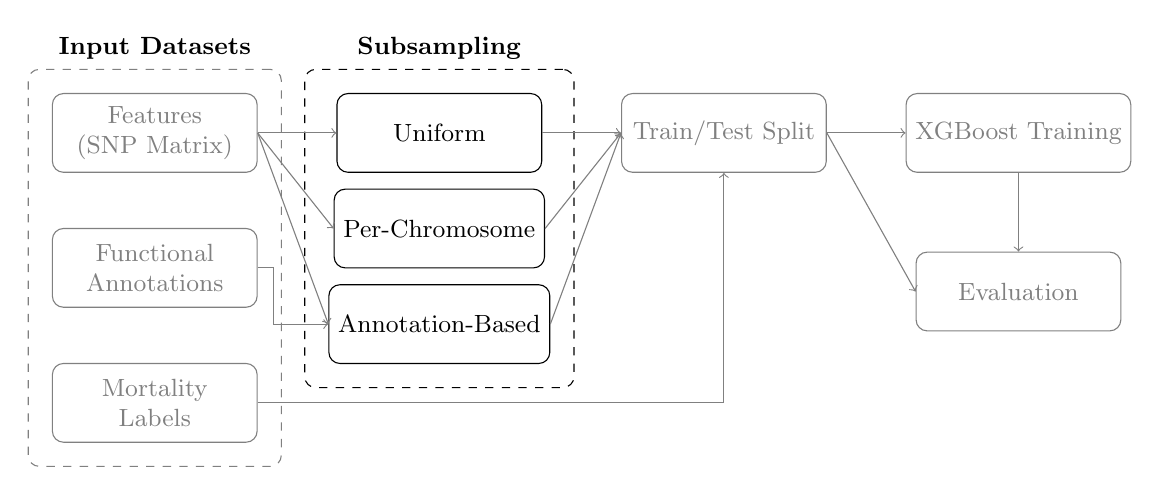
\begin{tikzpicture}[
        node distance=1cm and 0.1cm,
        every node/.style={font=\small},
        box/.style={draw, rectangle, rounded corners, minimum height=1cm, minimum width=2.6cm, align=center},
        group/.style={draw, rectangle, dashed, inner sep=0.3cm, rounded corners}
    ]

    \node[box, color=gray] (features) {Features \\ (SNP Matrix)};
    \node[box, color=gray, below=0.7cm of features] (annotation) {Functional \\ Annotations};
    \node[box, color=gray, below=0.7cm of annotation] (mortality) {Mortality \\ Labels};

    \node[group, color=gray, fit=(features)(mortality)(annotation), label=above:{\textbf{Input Datasets}}] (dataset_group) {};

    \node[box, right=1cm of features] (uniform) {Uniform};
    \node[box, below=0.2cm of uniform] (chr) {Per-Chromosome};
    \node[box, below=0.2cm of chr] (annot) {Annotation-Based};

    \node[group, fit=(uniform)(chr)(annot), label=above:{\textbf{Subsampling}}] (subsampling_group) {};

    \node[box, color=gray, right=1cm of uniform] (split) {Train/Test Split};
    \node[box, color=gray, right=1cm of split] (xgboost) {XGBoost Training};
    \node[box, color=gray, below=of xgboost] (evaluate) {Evaluation};

    \draw[->, color=gray] (features.east) -- ++(0.1,0) |- (uniform.west);
    \draw[->, color=gray] (features.east) -- (chr.west);
    \draw[->, color=gray] (features.east) -- (annot.west);

    \draw[->, color=gray] (annotation.east) -- ++(0.2,0) |- (annot.west);

    \draw[->, color=gray] (uniform.east) -- ++(0.1,0) |- (split.west);
    \draw[->, color=gray] (chr.east) -- (split.west);
    \draw[->, color=gray] (annot.east) -- (split.west);

    \draw[->, color=gray] (mortality.east) -| (split.south);

    \draw[->, color=gray] (split.east) -- (xgboost.west);
    \draw[->, color=gray] (split.east) -- (evaluate.west);
    \draw[->, color=gray] (xgboost.south) -- (evaluate.north);

    \end{tikzpicture}
\end{figure}
\end{frame}

\begin{frame}
\frametitle{Uniform Subsampling}
\begin{itemize}
  \item Randomly sample a fixed proportion $p$ of all SNPs.
  \item Simple but may cause imbalance across chromosomes.
\end{itemize}

\vspace{0.3cm}

\centering
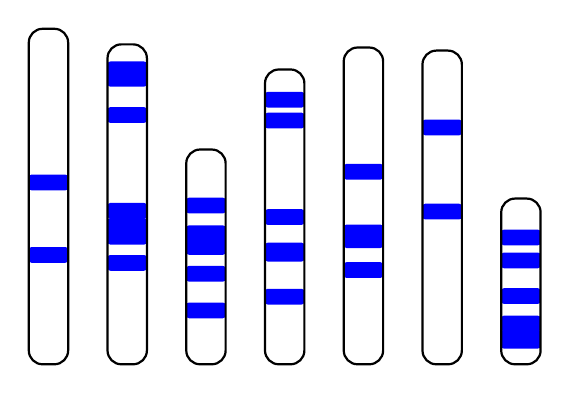
\begin{tikzpicture}
    \def\bars{7} % Number of bars
    \def\maxheight{2.5} % Max height of bars
    
    % Loop through each bar
    \foreach \i in {1,...,\bars} {
      \pgfmathsetmacro{\barheight}{2+rnd*\maxheight} % Random height for the bar
      \pgfmathsetmacro{\numsegments}{int(rnd*10)}
      
      % Position for the current bar
      \def\xpos{\i*1} % Space out the bars
      
      % Loop through each segment of the current bar
      \foreach \j in {1,...,\numsegments} {
        \pgfmathsetmacro{\segmentheight}{0.05+rnd*(\barheight-0.3)} % Random height for the segment
        
        % Draw the segment with random color
        \fill[blue, rounded corners=1pt] (\xpos, \segmentheight) rectangle (\xpos+0.5, \segmentheight+0.2);
      }
      
      \draw[thick, black, rounded corners=5pt] (\xpos, 0) rectangle (\xpos+0.5, \barheight+0.05);
    }
  \end{tikzpicture}
\end{frame}

\begin{frame}
\frametitle{Per-Chromosome Subsampling}
\begin{itemize}
  \item Ensures balanced representation from each chromosome.
  \item Randomly sample same number of SNPs per chromosome.
\end{itemize}

\vspace{0.3cm}

\centering
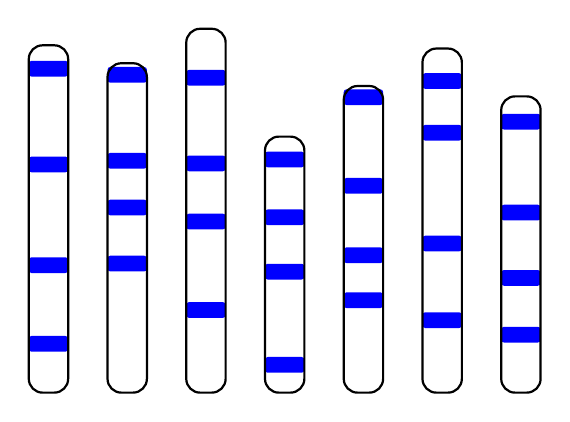
\begin{tikzpicture}
    \def\bars{7} % Number of bars
    \def\maxheight{2.5} % Max height of bars
    
    % Loop through each bar
    \foreach \i in {1,...,\bars} {
      \pgfmathsetmacro{\barheight}{2+rnd*\maxheight} % Random height for the bar
      \pgfmathsetmacro{\numsegments}{4}
      
      % Position for the current bar
      \def\xpos{\i*1} % Space out the bars
      
      % Loop through each segment of the current bar
      \pgfmathsetmacro{\minsegmentheight}{0.05}
      \pgfmathsetmacro{\j}{1}
        \pgfmathsetmacro{\segmentheight}{\minsegmentheight+rnd*(\barheight-\minsegmentheight-0.7*(\numsegments-\j))} % Random height for the segment
        
        % Draw the segment with random color
        \fill[blue, rounded corners=1pt] (\xpos, \segmentheight) rectangle (\xpos+0.5, \segmentheight+0.2);
        \pgfmathsetmacro{\minsegmentheight}{\segmentheight + 0.4}
      \pgfmathsetmacro{\j}{2}
        \pgfmathsetmacro{\segmentheight}{\minsegmentheight+rnd*(\barheight-\minsegmentheight-0.7*(\numsegments-\j))} % Random height for the segment
        
        % Draw the segment with random color
        \fill[blue, rounded corners=1pt] (\xpos, \segmentheight) rectangle (\xpos+0.5, \segmentheight+0.2);
        \pgfmathsetmacro{\minsegmentheight}{\segmentheight + 0.4}
      \pgfmathsetmacro{\j}{3}
        \pgfmathsetmacro{\segmentheight}{\minsegmentheight+rnd*(\barheight-\minsegmentheight-0.7*(\numsegments-\j))} % Random height for the segment
        
        % Draw the segment with random color
        \fill[blue, rounded corners=1pt] (\xpos, \segmentheight) rectangle (\xpos+0.5, \segmentheight+0.2);
        \pgfmathsetmacro{\minsegmentheight}{\segmentheight + 0.4}
      \pgfmathsetmacro{\j}{4}
        \pgfmathsetmacro{\segmentheight}{\minsegmentheight+rnd*(\barheight-\minsegmentheight-0.7*(\numsegments-\j))} % Random height for the segment
        
        % Draw the segment with random color
        \fill[blue, rounded corners=1pt] (\xpos, \segmentheight) rectangle (\xpos+0.5, \segmentheight+0.2);
        \pgfmathsetmacro{\minsegmentheight}{\segmentheight + 0.4}
      
      
      \draw[thick, black, rounded corners=5pt] (\xpos, 0) rectangle (\xpos+0.5, \barheight+0.2);
    }
  \end{tikzpicture}
\end{frame}

\begin{frame}
\frametitle{Annotation-Based Subsampling}
\begin{itemize}
  \item Filter SNPs by biological annotation.
  \item Then apply uniform subsampling to relevant regions.
\end{itemize}

\vspace{0.3cm}

%TODO change colors
\centering
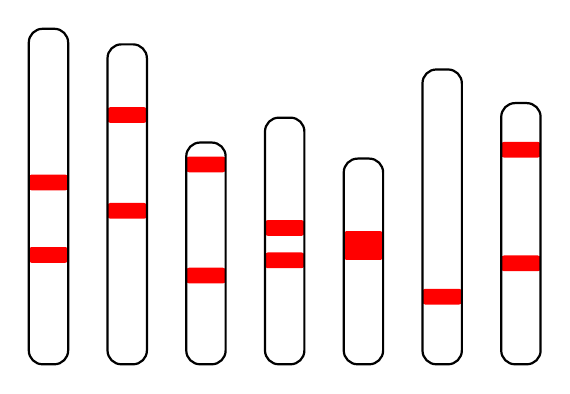
\begin{tikzpicture}
    \def\bars{7} % Number of bars
    \def\maxheight{2.5} % Max height of bars
    
    % Loop through each bar
    \foreach \i in {1,...,\bars} {
      \pgfmathsetmacro{\barheight}{2+rnd*\maxheight} % Random height for the bar
      \pgfmathsetmacro{\numsegments}{int(rnd*3)}
      
      % Position for the current bar
      \def\xpos{\i*1} % Space out the bars
      
      % Loop through each segment of the current bar
      \foreach \j in {1,...,\numsegments} {
        \pgfmathsetmacro{\segmentheight}{0.05+rnd*(\barheight-0.3)} % Random height for the segment
        
        % Draw the segment with random color
        \fill[red, rounded corners=1pt] (\xpos, \segmentheight) rectangle (\xpos+0.5, \segmentheight+0.2);
      }
      
      \draw[thick, black, rounded corners=5pt] (\xpos, 0) rectangle (\xpos+0.5, \barheight+0.05);
    }
  \end{tikzpicture}
\end{frame}

\begin{frame}{Parameter Evaluation}
\begin{figure}[htb!]
    \centering
    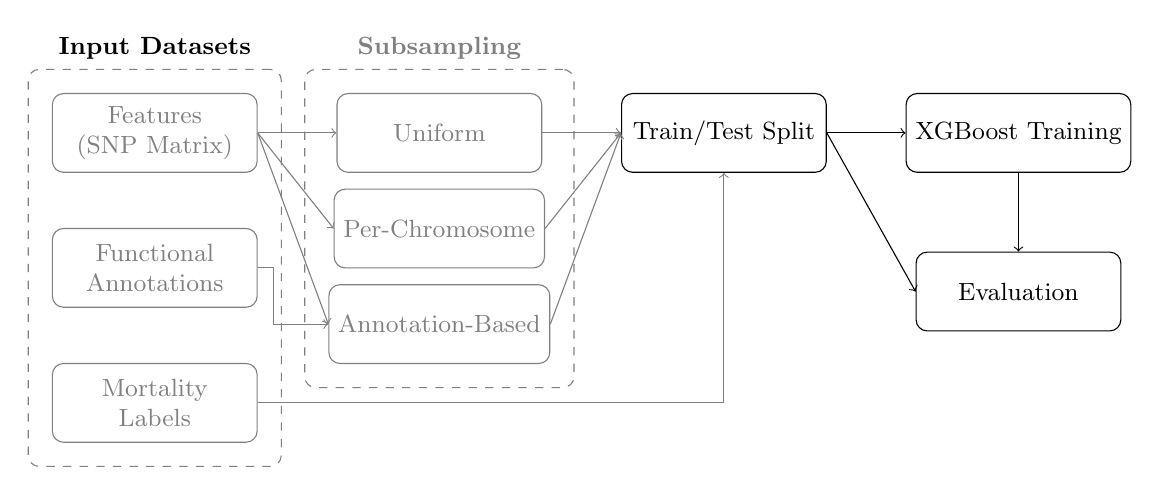
\begin{tikzpicture}[
        node distance=1cm and 0.1cm,
        every node/.style={font=\small},
        box/.style={draw, rectangle, rounded corners, minimum height=1cm, minimum width=2.6cm, align=center},
        group/.style={draw, rectangle, dashed, inner sep=0.3cm, rounded corners}
    ]

    \node[box, color=gray] (features) {Features \\ (SNP Matrix)};
    \node[box, color=gray, below=0.7cm of features] (annotation) {Functional \\ Annotations};
    \node[box, color=gray, below=0.7cm of annotation] (mortality) {Mortality \\ Labels};

    \node[group, color=gray, fit=(features)(mortality)(annotation), label=above:{\textbf{Input Datasets}}] (dataset_group) {};

    \node[box, color=gray, right=1cm of features] (uniform) {Uniform};
    \node[box, color=gray, below=0.2cm of uniform] (chr) {Per-Chromosome};
    \node[box, color=gray, below=0.2cm of chr] (annot) {Annotation-Based};

    \node[group, color=gray, fit=(uniform)(chr)(annot), label=above:{\textbf{\textcolor{gray}{Subsampling}}}] (subsampling_group) {};

    \node[box, right=1cm of uniform] (split) {Train/Test Split};
    \node[box, right=1cm of split] (xgboost) {XGBoost Training};
    \node[box, below=of xgboost] (evaluate) {Evaluation};

    \draw[->, color=gray] (features.east) -- ++(0.1,0) |- (uniform.west);
    \draw[->, color=gray] (features.east) -- (chr.west);
    \draw[->, color=gray] (features.east) -- (annot.west);

    \draw[->, color=gray] (annotation.east) -- ++(0.2,0) |- (annot.west);

    \draw[->, color=gray] (uniform.east) -- ++(0.1,0) |- (split.west);
    \draw[->, color=gray] (chr.east) -- (split.west);
    \draw[->, color=gray] (annot.east) -- (split.west);

    \draw[->, color=gray] (mortality.east) -| (split.south);

    \draw[->] (split.east) -- (xgboost.west);
    \draw[->] (split.east) -- (evaluate.west);
    \draw[->] (xgboost.south) -- (evaluate.north);

    \end{tikzpicture}
\end{figure}
\end{frame}
%TODO add cambio della guardia / sostanza

\begin{frame}
\frametitle{Control of Randomness}
In order to limit the variance of results we impose:
\begin{itemize}
  \item XGBoost random seed, train-test split fixed
  \item Subsampling is the only random component varying between experiments.
\end{itemize}
\vspace{0.3cm}
\centering
 \resizebox{0.8\textwidth}{!}{
    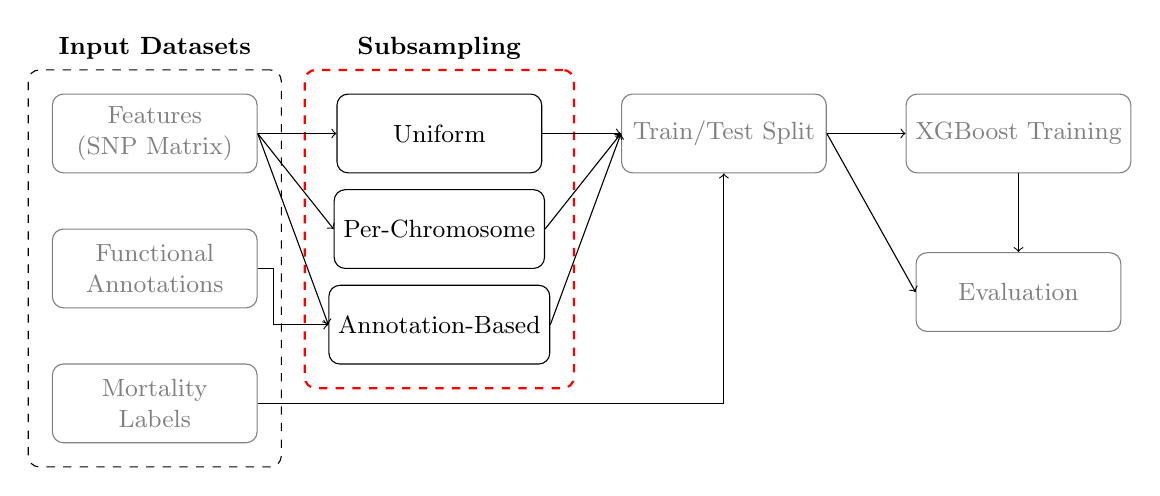
\begin{tikzpicture}[
        node distance=1cm and 0.1cm,
        every node/.style={font=\small},
        box/.style={draw, rectangle, rounded corners, minimum height=1cm, minimum width=2.6cm, align=center},
        group/.style={draw, rectangle, dashed, inner sep=0.3cm, rounded corners}
    ]

    \node[box, color=gray] (features) {Features \\ (SNP Matrix)};
    \node[box, color=gray, below=0.7cm of features] (annotation) {Functional \\ Annotations};
    \node[box, color=gray, below=0.7cm of annotation] (mortality) {Mortality \\ Labels};

    \node[group, fit=(features)(mortality)(annotation), label=above:{\textbf{Input Datasets}}] (dataset_group) {};

    \node[box, right=1cm of features] (uniform) {Uniform};
    \node[box, below=0.2cm of uniform] (chr) {Per-Chromosome};
    \node[box, below=0.2cm of chr] (annot) {Annotation-Based};

    \node[group, thick, color=red, fit=(uniform)(chr)(annot), label=above:{\textbf{Subsampling}}] (subsampling_group) {};

    \node[box, color=gray, right=1cm of uniform] (split) {Train/Test Split};
    \node[box, color=gray, right=1cm of split] (xgboost) {XGBoost Training};
    \node[box, color=gray, below=of xgboost] (evaluate) {Evaluation};

    \draw[->] (features.east) -- ++(0.1,0) |- (uniform.west);
    \draw[->] (features.east) -- (chr.west);
    \draw[->] (features.east) -- (annot.west);

    \draw[->] (annotation.east) -- ++(0.2,0) |- (annot.west);

    \draw[->] (uniform.east) -- ++(0.1,0) |- (split.west);
    \draw[->] (chr.east) -- (split.west);
    \draw[->] (annot.east) -- (split.west);

    \draw[->] (mortality.east) -| (split.south);

    \draw[->] (split.east) -- (xgboost.west);
    \draw[->] (split.east) -- (evaluate.west);
    \draw[->] (xgboost.south) -- (evaluate.north);

    \end{tikzpicture}
}
\end{frame}

\section{Results}
\begin{frame}
\frametitle{Subsampling Ratios and baseline results}
%TODO visualize multiple subsampling ratios
\begin{itemize}
    \item Subsampled with multiple $p$ values: log-spaced varying from the whole genome to few SNPs.
  \item Trained model for each combination of model and subsample rate.
  \item Multiple runs for each pair of parameters.
  \item Comparison with \textbf{baseline results} from a "dumb" classifier, always guessing the most common class.
\end{itemize}
\end{frame}

\begin{frame}{Results: uniform subsampling}
\begin{figure}[H]
    \centering
    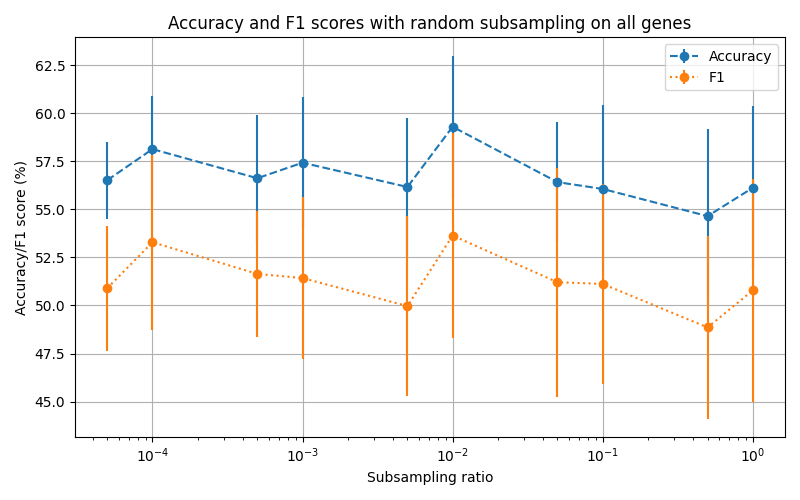
\includegraphics[height=0.5\textwidth]{../figures/subsample_plot.png}
    \caption{Plot of accuracy and F1 scores when subsampling uniformly on the whole genome.}
    \label{fig:res1a}
\end{figure}
\end{frame}

\begin{frame}{Results: uniform subsampling on each chromosome}
\begin{figure}[H]
    \centering
    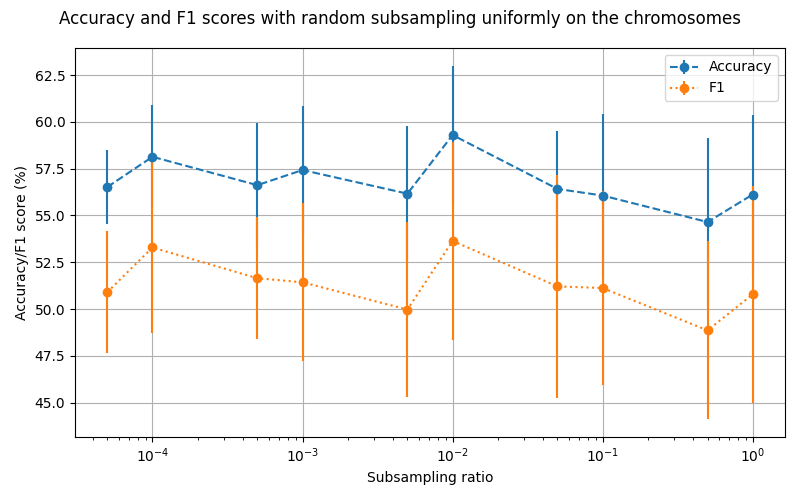
\includegraphics[height=0.5\textwidth]{../figures/uniform_sample_low_ratio.png}
    % \caption{Plot of accuracy and F1 scores when subsampling uniformly on each chromosome.}
    \label{fig:res1b}
\end{figure}
\end{frame}

\begin{frame}{Results: annotated subsampling (function)}
\begin{figure}[H]
    \centering
    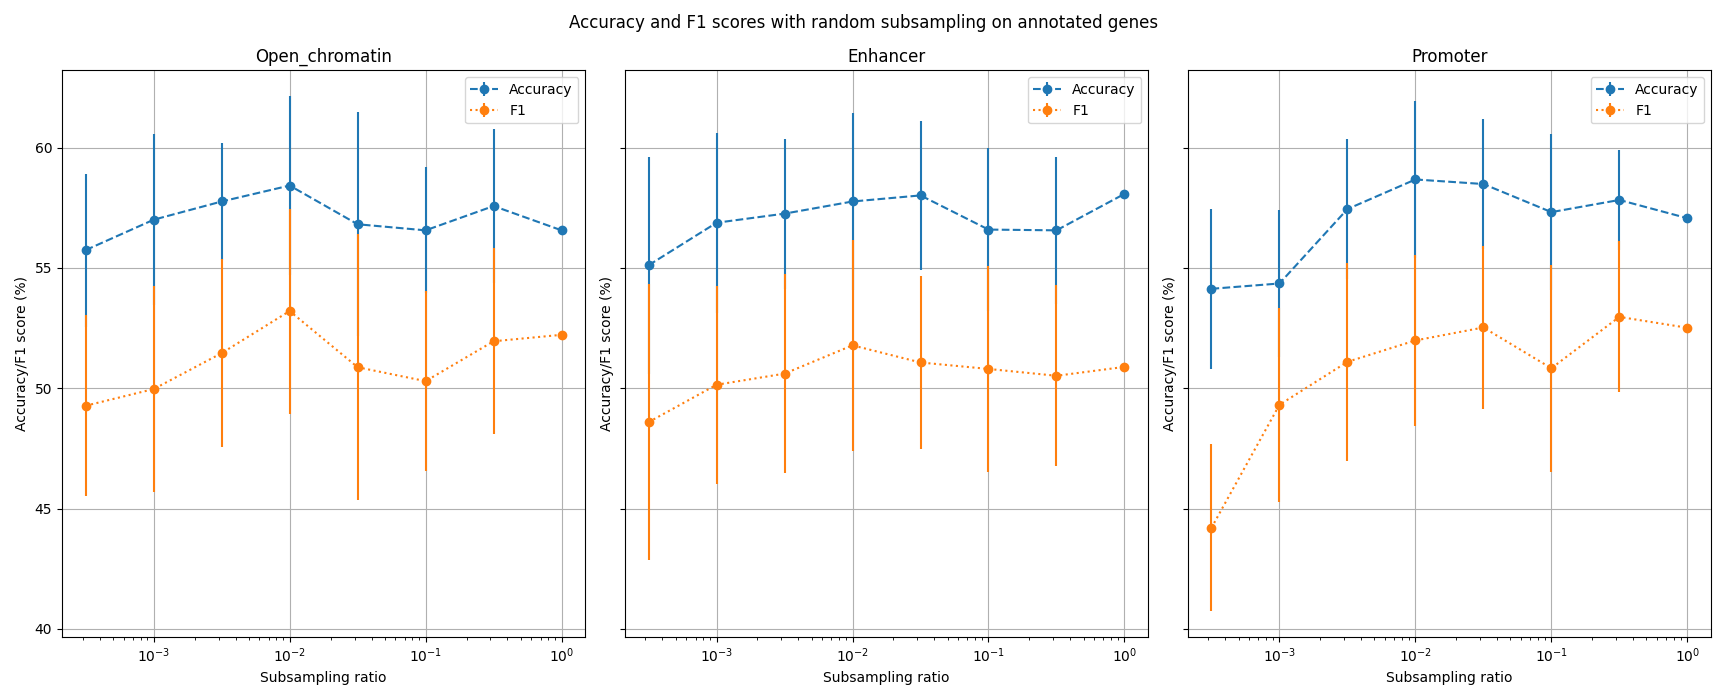
\includegraphics[width=\textwidth]{../figures/subsample_annotated.png}
    \label{fig:res2a}
\end{figure}
\end{frame}

\begin{frame}{Results: annotated subsampling (tissue number)}
\begin{figure}[H]
    \centering
    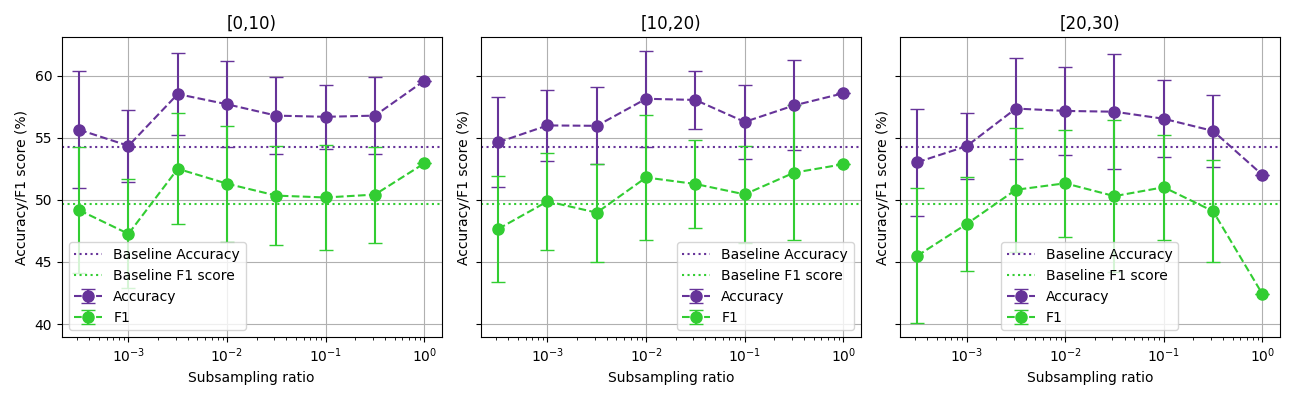
\includegraphics[width=\textwidth]{../figures/subsample_ntissue.png}
    \label{fig:res2b}
\end{figure}
\end{frame}

\section{Conclusions}
\begin{frame}
\frametitle{Conclusions}
\begin{minipage}{0.60\textwidth}
\begin{itemize}
  \item Random SNP subsampling retains model effectiveness.
  \item No strong trend between rate and accuracy (outside extremes): this may be good.
  \item There doesn't seem to be specific regions of the genome containing the information determining the disease effects.
\end{itemize}
\end{minipage}
\begin{minipage}{0.35\textwidth}
    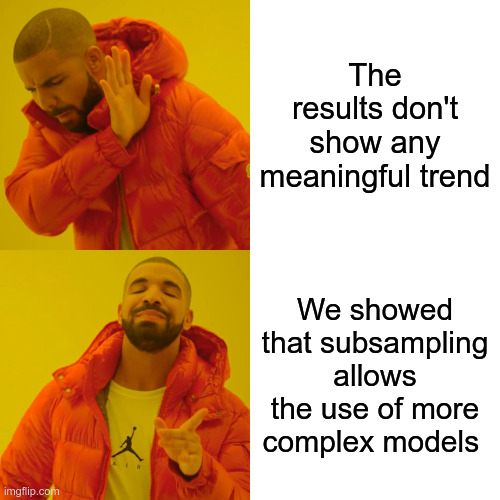
\includegraphics[width=0.99\textwidth]{memes/drake_results.jpg}
\end{minipage}
\end{frame}

\begin{emptyframe}
\centering
\Huge Thank You!
\end{emptyframe}

\end{document}
